
\section*{Learning Objectives}

\begin{itemize}
\item  Some basic computing constructs
\item  Moving beyond a graphical calculator
\item Getting started with debugging code in Julia
\end{itemize}

\section*{Outcomes} 
\begin{itemize}
\item Types of variables in Julia
\begin{itemize}
    \item Int64
    \item Float64
    \item Char
    \item String
    \end{itemize}
\item Building arrays
\item Declaring and plotting functions
\item Applying functions to arrays via broadcasting
\item First appearance of $n$-element Vector\{\texttt{Type}\} and $n \times m$
Matrix\{\texttt{Type}\}
\item Commenting out lines of code
\end{itemize}

\vspace*{1cm}

\textbf{Either download Lab1 from our Canvas site or open up a Jupyter notebook so that you can enter code as we go. It is suggested that you have line numbering toggled on.}  

\newpage

\section{Variable Types}

``A data \textbf{Type} or simply type is an attribute of data which tells the [computer] how the programmer intends to use the data \url{https://en.wikipedia.org/wiki/Data_type}". Computers have a limited amount of memory (zeros and ones) available to represent a number. If the computer knows that the number does not require a decimal point (as in -7, 0, 1, 45, etc,) then it can store it very compactly and hence store enormously large numbers of the \texttt{Int64 TYPE}. If the number requires a decimal to express it properly (such as pi, sqrt(2), 0.6) then Julia will store it in a different format. Mostly, Julia is able to handle the memory needs of our code without our help, because we tell Julia in advance the memory needs of our variables. \\

Everything in Julia has a \texttt{Type}. We will mostly use variables with these 4 \texttt{Type}
\begin{enumerate}
        \renewcommand{\labelenumi}{(\alph{enumi})}
        \setlength{\itemsep}{.1cm}
    \item \texttt{Int64}
    \item \texttt{Float64}
    \item \texttt{Char}
    \item \texttt{String}
\end{enumerate}

\texttt{\bf Int64} is used for integers or whole numbers, in other words, ...-3, -2, -1, 0, 1, 2, 3, ... The 64 refers to the number of 'bits', 0s and 1s, that are used to represent the number and its sign. The sign takes 1 bit, leaving 63 for the number. It is possible to represent numbers from $-2^{63}$ to $2^{63} - 1$. These are enormous values.\\

    
   \begin{figure}[hbt!]%
	\centering
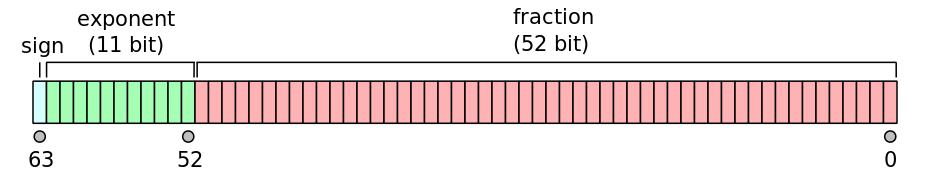
\includegraphics[width=0.75\columnwidth]{graphics/Chap02/FloatingPoint.png}
    \caption[]{ (Optional Read) Explanation from \url{https://en.wikipedia.org/wiki/Double-precision_floating-point_format} on how the bits used to represent a double-precision Floating Point number are organized in a computer.}
    \label{fig:FloatingPoint}
\end{figure} 


\texttt{\bf Float64} Floating point is computer speak for numbers that require decimal points, such as 1.414. Figure~\ref{fig:FloatingPoint} explains (optional read) why larger numbers can be stored in \texttt{Int64} than in \texttt{Float64}. We mostly do not care about this in ROB 101. We will primarily use floating point variables. But sometimes Julia really wants an integer variable and will throw a ``\texttt{Type Error}'' when you get it wrong. If you are not aware that all variables have a \texttt{Type}, then you will be at a loss to understand your mistake. \\

\texttt{\bf Char} is used to store characters, such as letters, numbers, or symbols. If you dig into Julia, you can learn how to use Chinese characters, Hebrew characters, Greek letters, and more. You place characters between single ` \hspace*{.3cm} ' marks, such as \texttt{x = `A'}.\\

\texttt{\bf String} is used for a sequence of characters in a single line. This could be a word, or a sentence, or even a number that is placed between double quote marks  ``\hspace*{.3cm}'', such as \texttt{myPlotTitle = ``My \#1  Plot in Julia''}.

\begin{rem}
Julia only prints out the last line in a cell that produces a result (it does not count a comment sign \# as a result). To cause other values to print to the screen, use the \texttt{@show} command. To verify (or learn) the \texttt{Type} of a variable, use the \texttt{typeof} command.
\end{rem}

% We will also use **TYPES** that are collections of the above types of variables, 
% - **Array** a collection of values that can be Int64, Float64, Char, String, etc.
% - **Vector** special kind of "one-dimensional'' array
% - **Matrix** special kind of array that can have many "dimensions''



\begin{lstlisting}[language=Julia,style=mystyle]
# Run me
w = 33
x = sqrt(2)
y = 'A'
z = "Oh oh, what I have I done!"
\end{lstlisting}
\textbf{Output} 
\begin{verbatim}
"Oh oh, what I have I done!"
\end{verbatim}



\begin{lstlisting}[language=Julia,style=mystyle]
# Run me
@show w = 33
@show x = sqrt(2)
@show y = 'A'
z = "Oh oh, what I have I done!"
\end{lstlisting}
\textbf{Output} 
\begin{verbatim}
w = 33 = 33
x = sqrt(2) = 1.4142135623730951
y = 'A' = 'A'
"Oh oh, what I have I done!"
\end{verbatim}

You could have added an \texttt{@show} command on $z$ as well. 
\begin{lstlisting}[language=Julia,style=mystyle]
@show typeof(w)
@show typeof(x)
@show typeof(y)
@show typeof(z)
\end{lstlisting}
\textbf{Output} 
\begin{verbatim}
typeof(w) = Int64
typeof(x) = Float64
typeof(y) = Char
typeof(z) = String

String
\end{verbatim}

\begin{rem}
 While Julia \url{https://docs.julialang.org/en/v1/base/numbers/#Standard-Numeric-Types} has a lot of number \texttt{TYPES}, it does not have all of the possible categories of numbers that mathematicians use, \url{https://youtu.be/5TkIe60y2GI}. In addition to \texttt{Int64} and \texttt{Float64}, we'll use from to time \texttt{Complex64}. 
\end{rem}

\section{Creating Simple Functions}

One of the main points of programming is the creation of new functions. Here, we'll learn the simplest way to create a function in Julia and then how to plot a graph of the function.

\begin{lstlisting}[language=Julia,style=mystyle]
f(x) = 5x^2 + 2x - 4  # this is too easy
\end{lstlisting}
\textbf{Output} 
\begin{verbatim}
f (generic function with 1 method)
\end{verbatim}

Note that we used \textbf{integer} coefficients when we composed the function.  
We can now evaluate the function at any point. Let's see what \texttt{Type} of variable is returned

\begin{lstlisting}[language=Julia,style=mystyle]
@show f(3)
@show f(3.0)
@show f(-pi)
\end{lstlisting}
\textbf{Output} 
\begin{verbatim}
f(3) = 47
f(3.0) = 47.0
f(-pi) = 39.06483669826721
39.06483669826721
\end{verbatim}
The first one is clearly \texttt{Int64} (there is no decimal point) and the other two are \texttt{Float64}. Next, we'll modify the function and make at least one of the coefficients a decimal number. All of the outputs are now type \texttt{Float64}.

\begin{lstlisting}[language=Julia,style=mystyle]
f(x) = 5.0x^2 + 2x - 4  # this is way too easy
@show f(3)
@show f(3.0)
f(-pi)
\end{lstlisting}
\textbf{Output} 
\begin{verbatim}
f(3) = 47.0
f(3.0) = 47.0
39.06483669826721
\end{verbatim}

\section{Very Basic Plotting}
\label{sec:basicPlotting}

\textbf{Rich source of plotting examples:} \url{https://gist.github.com/gizmaa/7214002} \\

\textbf{``Tutorial'' for plotting in Julia:} \url{https://docs.juliaplots.org/latest/tutorial/}\\

Julia attempts to avoid filling the memory of your computer with functionality that you do not intend to use. It does that through the use of \textbf{packages}, which are collections of useful functions designed around a single theme, such as plotting (package is called Plots), random numbers (package is called Random), or linear algebra (package is called LinearAlgebra). We have pre-loaded a bunch of packages into the ROB 101 Julia installation. The process of accessing packages is a bit different if you are working in a personal Julia installation versus the course site; we'll give both methods. In the course site, 
\begin{lstlisting}[language=Julia,style=mystyle]
# Turning on the plotting functions
using Plots
gr()
\end{lstlisting}
\textbf{Output} 
\begin{verbatim}
Plots.GRBackend()
\end{verbatim}
while if you are in a personal installation of Julia, do this
\begin{lstlisting}[language=Julia,style=mystyle]
# For a personal installation the first time you use a package
using Pkg
Pkg.add("Plots")
# After the first time, you just need to run these two commands
using Plots
gr()
\end{lstlisting}
\textbf{Output} 
\begin{verbatim}
Plots.GRBackend()
\end{verbatim}

We assume the function $f$ has already been defined. Here we are using $f(x) = 5.0x^2 + 2x - 4 $

\begin{lstlisting}[language=Julia,style=mystyle]
# Run me
# now, we can use the plot() function
plot(f, -5, 5, legend=false)  #f will be plotted for x varying from -5 to 5
\end{lstlisting}

\textbf{Output} 

	\begin{center}
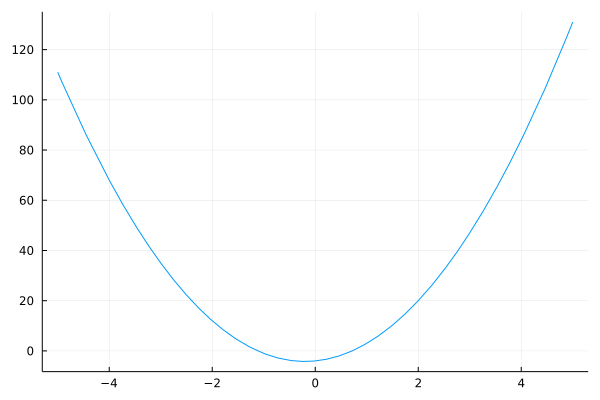
\includegraphics[width=0.5\columnwidth]{graphics/Chap02/Lab01_QuadraticNoLabels.png}
\end{center}

We can add labels to the plot
\begin{lstlisting}[language=Julia,style=mystyle]
plot!(xlabel = "x", ylabel = "y") # plot! modifies the previous plot
\end{lstlisting}

\textbf{Output} 

	\begin{center}
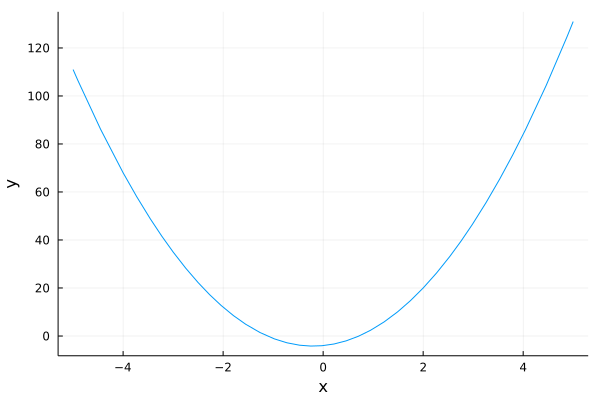
\includegraphics[width=0.5\columnwidth]{graphics/Chap02/Lab01_QuadraticWithLabels.png}
\end{center}


We can put all the commands in one line if we want
\begin{lstlisting}[language=Julia,style=mystyle]
# Run me
xmin=-5
xmax = 5
# You can add a bunch of stuff in one command line, if you want....
plot(f, xmin, xmax, xlabel = "x", ylabel = "y", legend = false) 
\end{lstlisting}

\textbf{Output} 

	\begin{center}
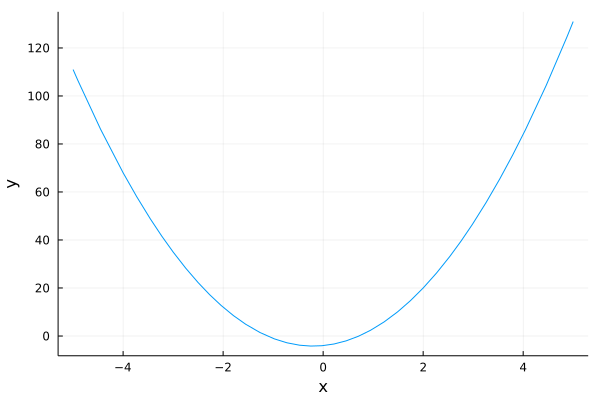
\includegraphics[width=0.5\columnwidth]{graphics/Chap02/Lab01_QuadraticWithLabels.png}
\end{center}



\begin{lstlisting}[language=Julia,style=mystyle]
# Run me to see how to have two functions on the same plot
f(x) = .1x^3 + 2
g(x) = x^2*sin(3*x) 
xmin = -2*pi
xmax = 2 *pi
titre = "Another Passable but not so Aesthetic Plot"
plot(f, xmin,xmax, title=titre, linewidth=3) 
# If you leave off the ! (bang), then the previous plot is erased and
# a new one is started. Try it.
plot!(g, xmin,xmax, title=titre, linewidth=3) #plot bang, it's kind of joyous!
println("Every point where the graphs of f and g cross is a solution of the equation f(x) - g(x) = 0")
plot!(xlabel = "x", ylabel = "y") # plot! modifies the previous plot
# png("Lab01_TwoFunctionsSameGraph") #Creates a png of the graph, uncomment to use
\end{lstlisting}
\textbf{Output} 
\begin{verbatim}
Every point where the graphs of f and g cross is a solution of the equation f(x) - g(x) = 0
\end{verbatim}
	\begin{center}
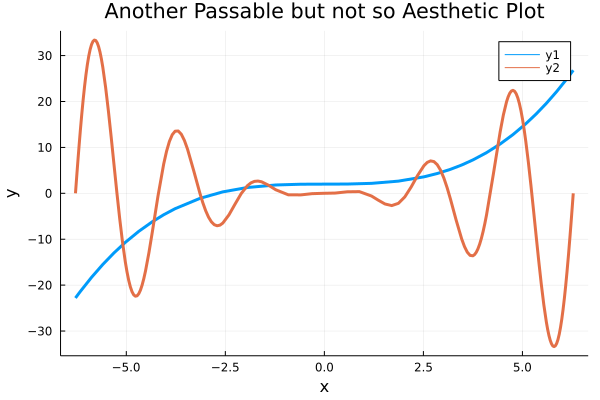
\includegraphics[width=0.5\columnwidth]{graphics/Chap02/Lab01_TwoFunctionsSameGraph.png}
\end{center}

\begin{lstlisting}[language=Julia,style=mystyle]
# Run me to see how to place two functions on the same plot
f(x) = .1x^3 + 2
g(x) = x^2*sin(3*x) 
xmin = -2*pi
xmax = 2 *pi
titre = "Another Passable but not so Aesthetic Plot"
plot([f,g], xmin,xmax, title=titre, linewidth=3) 
println("Every point where the graphs of f and g cross is a solution of the equation f(x) - g(x) = 0")
plot!(xlabel = "x", ylabel = "y") # plot! modifies the previous plot
\end{lstlisting}
\textbf{Output}   Same as from the previous cell.\\

Plotting in Julia is a bit awkward, in your instructor's opinion. We will mostly give you the plotting commands throughout the term. We'd rather you focus on other aspects of coding that are common to most programming languages. \\

\begin{center}
\fbox{ 
\textbf{To learn more about plotting in Julia:}  \url{https://docs.juliaplots.org/latest/tutorial/}}
\end{center}

\section{Creating Arrays}

An \textbf{array} ``is a data structure, which can store a fixed-size collection of elements of the same data type. An array is used to store a collection of data, but it is often more useful to think of an array as a collection of variables of the same type.'' \url{https://www.tutorialspoint.com/computer_programming/computer_programming_arrays.htm}. See also \url{https://press.rebus.community/programmingfundamentals/chapter/arrays-and-lists/}.\\

We will mostly be creating arrays with elements that are one of the following \texttt{Types}:
\begin{enumerate}
        \renewcommand{\labelenumi}{(\alph{enumi})}
        \setlength{\itemsep}{.1cm}
    \item \texttt{Int64}
    \item \texttt{Float64}
    \item \texttt{String}
\end{enumerate}

We'll first build an array with elements in a single row. 
\begin{lstlisting}[language=Julia,style=mystyle]
# Run me to create an array of 10 numbers
# a Matrix is one kind of array
# 1 x 10 Matrix{Int64} means it has one row and ten columns, 
# with each entry of TYPE Int64
myArray = [1 2 3 4 5 6 7 8 9 10]
\end{lstlisting}
\textbf{Output} 
\begin{verbatim}
1×10 Matrix{Int64}:
 1  2  3  4  5  6  7  8  9  10
\end{verbatim}

Note that in Julia, what we call a \textbf{row vector} in lecture is being called a $1 \times n$ matrix, where in this case $n=10$ because there are 10 entries in the vector. Note that Julia is confirming the data \texttt{Type} for us, $ 1 \times 10 ~\text{\rm  Matrix}\{\bf Int64\}.$ Each entry of the array has data type \texttt{\bf Int64}. However, if we change even one of the entries to \texttt{\bf Float64}, then \textbf{all of the entries} become \texttt{\bf Float64}, as shown below.

\begin{lstlisting}[language=Julia,style=mystyle]
# Run me to create an array of 10 numbers
# We change one of the values to a number of TYPE Float64, 
# and leave the rest as TYPE Int64. Watch what happens
# 
# 1 x 10 Matrix{Float64} means it has one row and ten columns, 
# with each entry of TYPE Float64
println("All elements assume TYPE Float64")
myArray = [1.0 2 3 4 5 6 7 8 9 10]
\end{lstlisting}
\textbf{Output} 
\begin{verbatim}
All elements assume TYPE Float64

1 x 10 Matrix{Float64}:
 1.0  2.0  3.0  4.0  5.0  6.0  7.0  8.0  9.0  10.0
\end{verbatim}

In Julia, arrays that are arranged in a column are called \textbf{Vectors}. What we call a \textbf{column vector} in lecture is simply a vector in Julia because Julia does not have two kinds of vectors. Julia only has column vectors and because of that, it is redundant to use the adjective ``column''. OK! In lecture, it is not redundant to specify column vs row when talking about a vector.\\

In Julia, when you use \textbf{commas} or \textbf{semicolons} to separate the elements of an array to form a ``column vector'', it is automatically declared as a \textbf{Vector}. Below, we build a 
5-element \texttt{Vector\{\bf Float64\}}. We used semicolons. You can replace the semicolons with commas and check that you get the same result. You cannot mix, however, commas and semicolons in the same array. 

\begin{lstlisting}[language=Julia,style=mystyle]
# Run me to create an array of 5 numbers
# arranged as a column
# 5-element Vector{Float64} means it has five elements, 
# each with value of TYPE Float64
#
println("You can separate the elements by commas OR by semicolons. This is different than MATLAB.")
myArray = [1.0; 2; 3; 4; 5]
\end{lstlisting}
\textbf{Output} 
\begin{verbatim}
You can separate the elements by commas OR by semicolons. This is different than MATLAB.

5-element Vector{Float64}:
 1.0
 2.0
 3.0
 4.0
 5.0
\end{verbatim}

You can build vectors with elements that have type \texttt{String}.

\begin{lstlisting}[language=Julia,style=mystyle]
# Run me to create an array with names in it
# 6-element Vector{String} means it is a column vector with 
# elements of TYPE String. Note that we used commas this time.
animalsVector = ["lemur", "elephant", "tiger", "panda", "zebra", "cuttlefish"]
\end{lstlisting}
\textbf{Output} 
\begin{verbatim}
6-element Vector{String}:
 "lemur"
 "elephant"
 "tiger"
 "panda"
 "zebra"
 "cuttlefish"
\end{verbatim}

You can also create $1 \times n$ matrices with elements that have type \texttt{String}.

\begin{lstlisting}[language=Julia,style=mystyle]
# Run me to see what happens when one uses spaces to separate the elements
animalsVector = ["lemur" "elephant" "tiger" "panda" "zebra" "cuttlefish"]
\end{lstlisting}
\textbf{Output} 
\begin{verbatim}
1×6 Matrix{String}:
 "lemur"  "elephant"  "tiger"  "panda"  "zebra"  "cuttlefish"
\end{verbatim}

\begin{exercise}
Build three arrays, each with five elements
\begin{enumerate}
    \item myArray01 is a 1 x 5 matrix with entries of TYPE Float64
    \item myArray02 is a 5-element vector with entries of TYPE Float64
    \item myArray03 is a 5-element vector with entries of TYPE String
\end{enumerate}
\end{exercise}
\textbf{Solution}


\begin{lstlisting}[language=Julia,style=mystyle]
# Place your answers here
@show myArray01 = [1/3 11 4 2^(0.5) 7.62]
@show myArray02 = [1/3; 11; 4; 2^(0.5); 7.62]
myArray03 = ["un"; "deux"; "trois"; "quatre"; "cinque"]
\end{lstlisting}
\textbf{Output} 
\begin{verbatim}
myArray01 = [1 / 3 11 4 2 ^ 0.5 7.62] = [0.3333333333333333 11.0 4.0 1.4142135623730951 
7.62]

myArray02 = [1 / 3; 11; 4; 2 ^ 0.5; 7.62] = [0.3333333333333333, 11.0, 4.0, 
1.4142135623730951, 7.62]

5-element Vector{String}:
 "un"
 "deux"
 "trois"
 "quatre"
 "cinque"
\end{verbatim}

\section{Commenting out Lines of Code or Providing Explanations}


\begin{lstlisting}[language=Julia,style=mystyle]
# The pound sign comments out a single line
# x = 3
\end{lstlisting}
\textbf{Output} 
\begin{verbatim}
(nothing)
\end{verbatim}


\begin{lstlisting}[language=Julia,style=mystyle]
#
# Below is how you comment out multiple lines at one time
#=
enter comments or code here
it can take as many 
lines as you want
=#
\end{lstlisting}
\textbf{Output} 
\begin{verbatim}
(nothing)
\end{verbatim}

At least on a PC, you can highlight a section of code with your mouse\\

\setlength{\fboxrule}{3pt}%
	\centerline{ \fbox{ 
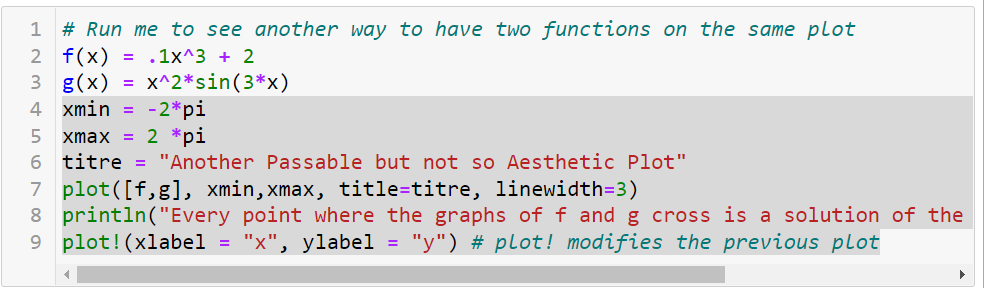
\includegraphics[width=0.9\columnwidth]{Chap02/MultiLineCommentingOut.png}}%
}

and then hit \texttt{Ctrl\,$/$} control-forward-slash (simultaneously) to comment out or un-comment multiple lines at a time. \\

\setlength{\fboxrule}{3pt}%
	\centerline{ \fbox{ 
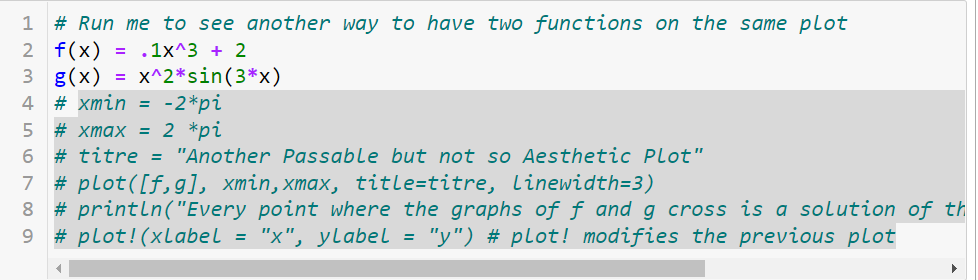
\includegraphics[width=0.9\columnwidth]{Chap02/MultiLineCommentingOut2.png}}%
}


\section{Applying Functions to Arrays via Broadcasting}

Julia has a special syntax for applying functions to individual elements of arrays. You need to add a ``dot'' after the function and before the argument to the function. It's best understood by doing it. 

\begin{lstlisting}[language=Julia,style=mystyle]
x = [0 pi/4 pi/2 3pi/4 pi 5pi/4]
\end{lstlisting}
\textbf{Output} 
\begin{verbatim}
1×6 Matrix{Float64}:
 0.0  0.785398  1.5708  2.35619  3.14159  3.92699
\end{verbatim}

\begin{lstlisting}[language=Julia,style=mystyle]
sin.(x)  # note the dot
\end{lstlisting}
\textbf{Output} 
\begin{verbatim}
1×6 Matrix{Float64}:
 0.0  0.707107  1.0  0.707107  1.22465e-16  -0.707107
\end{verbatim}

This also works with functions that you write yourself! It pretty awesome.

\begin{lstlisting}[language=Julia,style=mystyle]
f(x) = 1 + 2x + sin(x^2)
\end{lstlisting}
\textbf{Output} 
\begin{verbatim}
f (generic function with 1 method)
\end{verbatim}

\begin{lstlisting}[language=Julia,style=mystyle]
f.(x)  # note the dot
\end{lstlisting}
\textbf{Output} 
\begin{verbatim}
1×6 Matrix{Float64}:
 1.0  3.14927  4.76586  5.04438  6.85288  9.13678
\end{verbatim}

For an array,  $x = [x_1 ~~ x_2 ~~\ldots~~ x_n ]$, the returned value is $f.(x)=[f(x_1)~~  f(x_2)~~ \ldots ~~f(x_n)]$. This feature is called ``broadcasting''. If you leave out the ``dot'', this is what you get

\begin{lstlisting}[language=Julia,style=mystyle]
f(x)
\end{lstlisting}
\textbf{Output} 
\begin{verbatim}
DimensionMismatch("A has dimensions (1,6) but B has dimensions (1,6)")

Stacktrace:
  [1] gemm_wrapper!(C::Matrix{Float64}, tA::Char, tB::Char, A::Matrix{Float64},
  B::Matrix{Float64}, _add::LinearAlgebra.MulAddMul{true, true, Bool, Bool})
    @ LinearAlgebra /buildworker/worker/package_linux64/build/usr/share/julia/stdlib/
    v1.6/LinearAlgebra/src/matmul.jl:643
  [2] mul!
    @ /buildworker/worker/package_linux64/build/usr/share/julia/stdlib/v1.6/
    LinearAlgebra/src/matmul.jl:169 [inlined]
  [3] mul!
    @ /buildworker/worker/package_linux64/build/usr/share/julia/stdlib/v1.6/
    LinearAlgebra/src/matmul.jl:275 [inlined]
  [4] *
    @ /buildworker/worker/package_linux64/build/usr/share/julia/stdlib/v1.6/
    LinearAlgebra/src/matmul.jl:160 [inlined]
  [5] power_by_squaring(x_::Matrix{Float64}, p::Int64)
    @ Base ./intfuncs.jl:261
  [6] ^
    @ /buildworker/worker/package_linux64/build/usr/share/julia/stdlib/v1.6/
    LinearAlgebra/src/dense.jl:442 [inlined]
  [7] macro expansion
    @ ./none:0 [inlined]
  [8] literal_pow
    @ ./none:0 [inlined]
  [9] f(x::Matrix{Float64})
    @ Main ./In[8]:1
 [10] top-level scope
    @ In[10]:1
 [11] eval
    @ ./boot.jl:360 [inlined]
 [12] include_string(mapexpr::typeof(REPL.softscope), mod::Module, code::String,
 filename::String)
    @ Base ./loading.jl:1094

\end{verbatim}

You can also use the ``dot'' with addition or multiplication. Below, we add one to each entry of the array \texttt{x}. \\

\begin{lstlisting}[language=Julia,style=mystyle]
x .+ 1
\end{lstlisting}
\textbf{Output} 
\begin{verbatim}
1×6 Matrix{Float64}:
 1.0  1.7854  2.5708  3.35619  4.14159  4.92699
\end{verbatim}

The following code multiplies the entries of \texttt{x} times the corresponding entries in $y$,\\

\begin{lstlisting}[language=Julia,style=mystyle]
x = [1 2 3 4 5]
y = [5 4 3 2 1]
x.*y  # note the dot
\end{lstlisting}
\textbf{Output} 
\begin{verbatim}
1×5 Matrix{Int64}:
 5  8  9  8  5
\end{verbatim}

The same applies to squaring the entries of an array, such as \\

\begin{lstlisting}[language=Julia,style=mystyle]
x.^2  # note the dot
\end{lstlisting}
\textbf{Output} 
\begin{verbatim}
1×5 Matrix{Int64}:
 1  4  9  16  25
\end{verbatim}

The following applies the function $f(x)$ to each entry of \texttt{x} and then multiplies each entry of the resulting array times the corresponding entry in \texttt{y}.\\

\begin{lstlisting}[language=Julia,style=mystyle]
z=f.(x).*y  # we used two dots
\end{lstlisting}
\textbf{Output} 
\begin{verbatim}
1×5 Matrix{Float64}:
 19.2074  16.9728  22.2364  17.4242  10.8676
\end{verbatim}

The following applies the function $f(x)$ to each entry of \texttt{x}, then multiplies each entry of the resulting array times the corresponding entry in \texttt{y}, and finally adds 2 to each entry.\\

\begin{lstlisting}[language=Julia,style=mystyle]
z=f.(x).*y .+ 2  # we used three dots
\end{lstlisting}
\textbf{Output} 
\begin{verbatim}
1×5 Matrix{Float64}:
 21.2074  18.9728  24.2364  19.4242  12.8676
\end{verbatim}

\vspace*{.2cm}

\begin{center}
\fbox{ 
\textbf{
We note that $z = [z_1~~ z_2 ~~ \ldots~~ z_n]$, where for $1 \le i \le n$, the components of $z$ are given by $z_i = f(x_i)*y_i+ 2$.
}
}
\end{center}


% For emphasis, we note that $z = [z_1~~ z_2 ~~ \ldots~~ z_n]$, where for $1 \le i \le n$, the components of $z$ are given by $z_i = f(x_i)*y_i+ 2$.

\section{Debugging}

We created our first function in Chapter~\ref{sec:basicPlotting}. Here we'll show a common programming error that you might think is a bug.

\begin{lstlisting}[language=Julia,style=mystyle]
g=2 # set the variable g to a constant
\end{lstlisting}
\textbf{Output} 
\begin{verbatim}
2
\end{verbatim}

That's pretty simple! Now, imagine that you used the variable $g$ 15 cells back and have completely forgotten about it. You then want to create a function and call it $g$. 
\begin{lstlisting}[language=Julia,style=mystyle]
g(x) = 5x + 2
\end{lstlisting}
\textbf{Output} 
\begin{verbatim}
cannot define function g; it already has a value

Stacktrace:
 [1] top-level scope
   @ none:0
 [2] top-level scope
   @ In[4]:1
 [3] eval
   @ ./boot.jl:360 [inlined]
 [4] include_string(mapexpr::typeof(REPL.softscope), mod::Module, 
 code::String, filename::String)
   @ Base ./loading.jl:1094

\end{verbatim}

In the example, Cell [4] is the cell where we defined $g(x)$. There are two cures for this:
\begin{itemize}
    \item Clear your Kernel, \textbf{which will erase the variables in your Jupyter notebook without erasing your code}. You can then run the cell above again and it will work fine.

    \item Choose a different name for the function, which we illustrate below.
\end{itemize}
\begin{lstlisting}[language=Julia,style=mystyle]
g2(x) = 5x + 2
\end{lstlisting}
\textbf{Output} 
\begin{verbatim}
g2 (generic function with 1 method)
\end{verbatim}

\vspace*{.2cm}

\begin{tcolorbox}[title={\large \bf Debugging}]

    \begin{itemize}
        \item Taken From the Pro-tip page at Georgia Tech for a graduate-level course: \url{https://cse6040.gatech.edu/fa22/pro_tips.html}

        \item Debugging is an iterative process where you must trace the undesired behavior back to the root cause. Sometimes it's simple; other times it can be frustratingly complex.

        \item Identify what is wrong. This needs to be as precise as possible. If you don't understand the error in the traceback - Google it!. Check the syntax, parameters, and inputs of any function calls.

        \item Identify where the wrong thing got set. This will usually be an assignment or a function call.

        \item Rinse and repeat until you have found and corrected the root cause.
    \end{itemize}
\end{tcolorbox}